%%%%%%%%%%%%%%%%%%%%%%%%%%%%%%%%%%%%%%%%%%%%%%%%%%%%%%%%%%%%%%%%%%%%%%%
% Project Name : HyperPath                                            %
% Project Home : https://github.com/TeamAC/HyperPath                  %
% Part         : Bibliography                                         %
% Author       : chedi                                                %
% Comments     :                                                      %
%                                                                     %
%%%%%%%%%%%%%%%%%%%%%%%%%%%%%%%%%%%%%%%%%%%%%%%%%%%%%%%%%%%%%%%%%%%%%%%


\section{Server Application}

  \begin{figure}[p]
    \begin{center}
      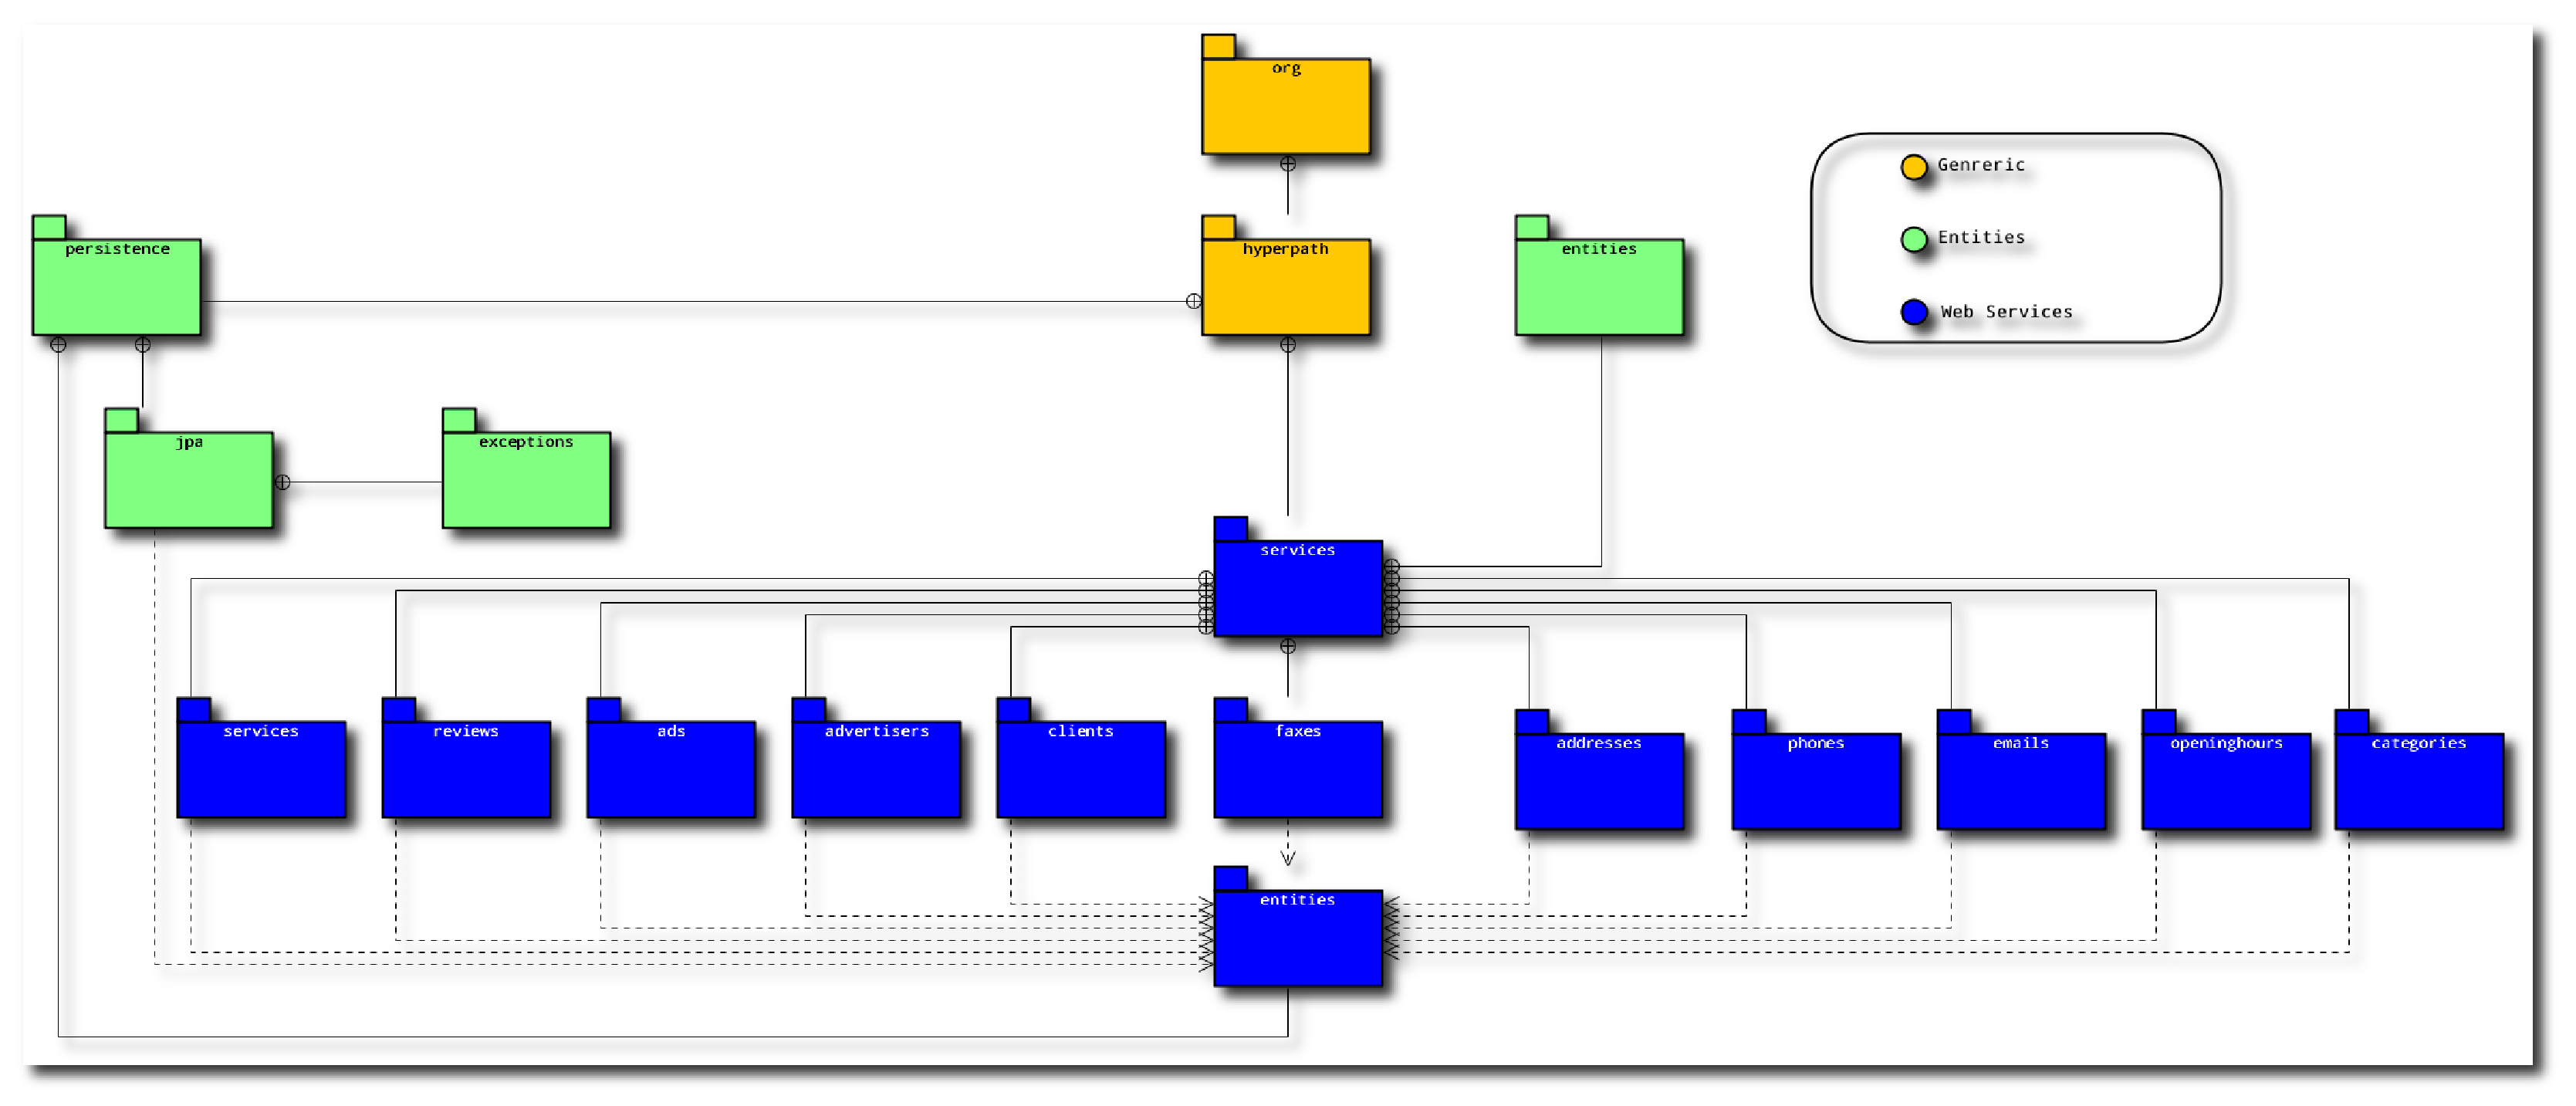
\includegraphics[scale=0.5]{Figures/HyperPath_server_packages.eps}
     \end{center}
     \caption{Server package architecture}
     \label{Server package architecture}
  \end{figure}
\pagebreak
\section{Data model}
Using the client server application, we deployed a EJB on the glassfish Java
application server to manage all the data model using JPA persistence. For that
perpuse we created two main packages under org.hyperpath.persistence:
\begin{description}
  \item[jpa: ] this package contains all the jpa controller nedded to manage the
  data model
  \item[entities: ] this package holds the entities class mapping the data model
\end{description}

  \begin{figure}[p]
    \begin{center}
      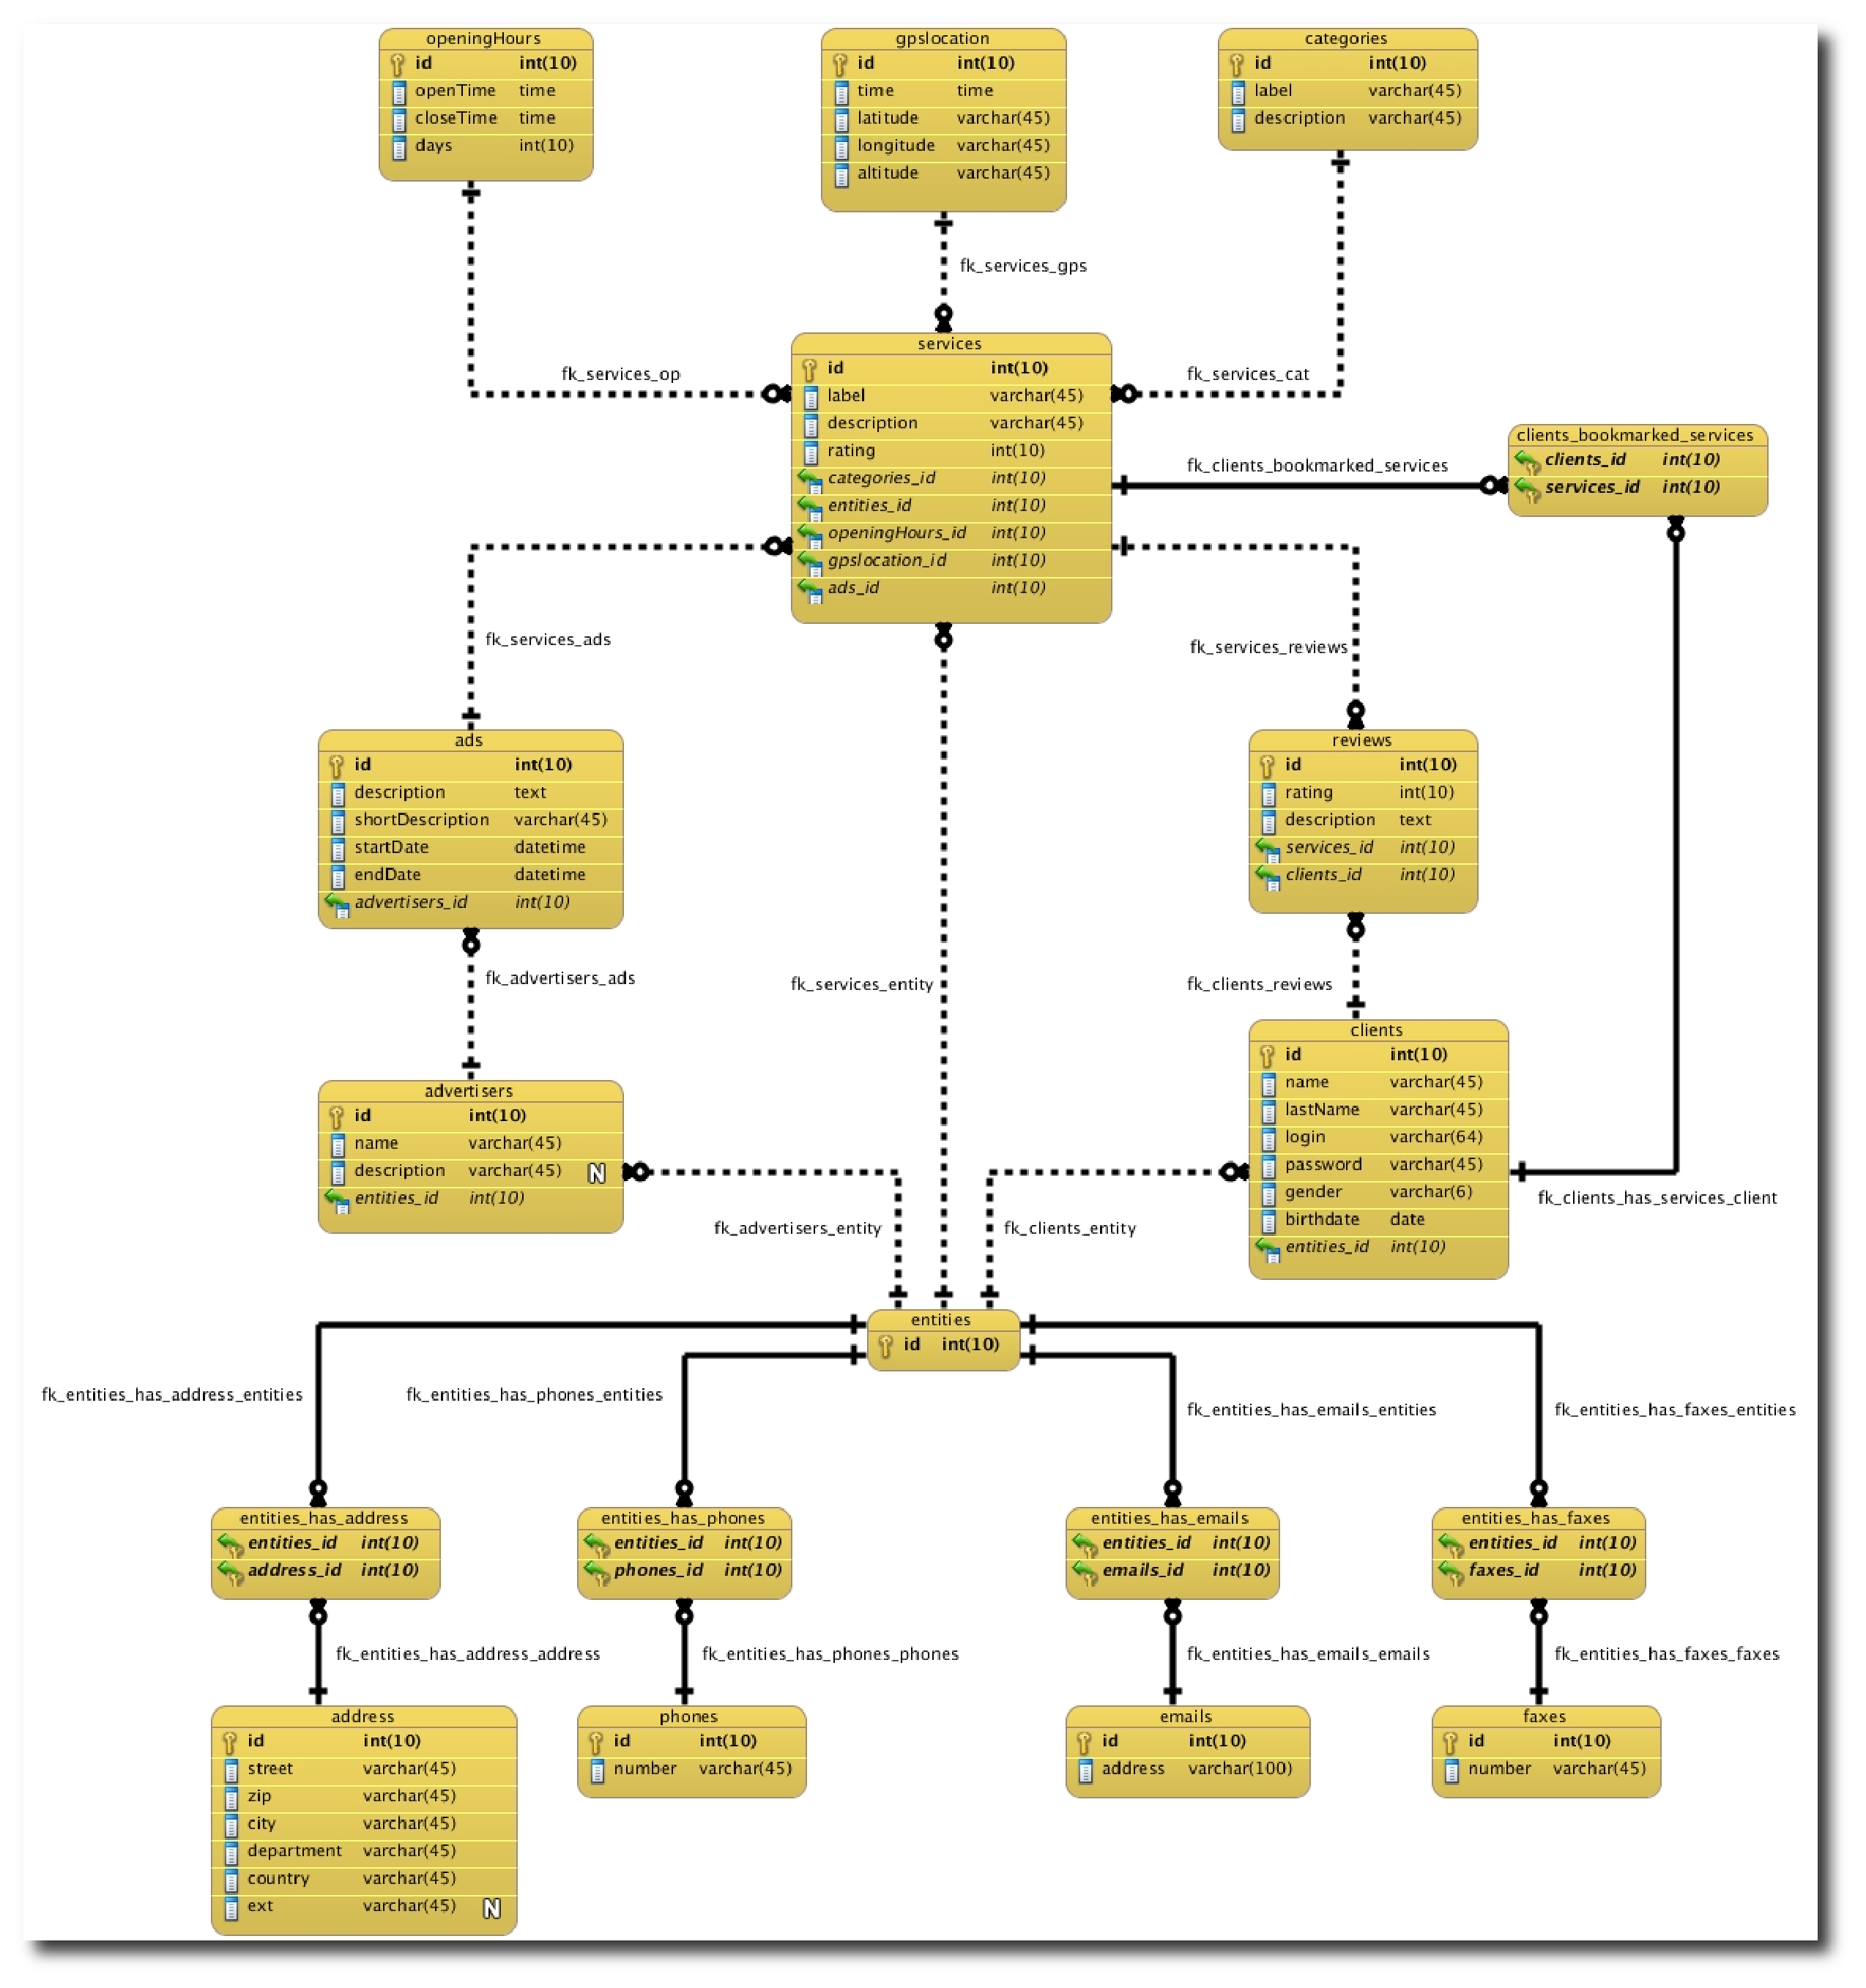
\includegraphics[scale=0.4]{Figures/HyperPathServerEntities.eps}
     \end{center}
     \caption{Server application entities}
     \label{Server application entities}
  \end{figure}
\pagebreak

\section{Client application}